\chapter{LV 8 am 27.06.2014}
\section{Verifikation vs. Validierung}
\paragraph{Verifikation}
Bei der Verifikation überprüft man die Software gegen ihre Spezifikation.
\begin{itemize}
\item Sind die Spezifikationen richtig umgesetzt?
\item Wurde das Produkt richtig erstellt?
\end{itemize}

\paragraph{Validierung}
Bei der Validierung überprüft man die Software gegen ihre Anforderungen und Erwartungen ihrer Benutzer.
\begin{itemize}
\item Wurde das richtige Produkt erstellt?
\item Wurden die Benutzeranforderungen richtig und vollständig erfasst, verstanden und in der Spezifikation umgesetzt?
\end{itemize}

Die Verifikation und Validierung von Software können in dem Maße als äquivalent betrachtet werden, wenn die Anforderungen der Benutzer richtig und vollständig verstanden und dokumentiert und korrekt und vollständig in der Spezifikation berücksichtigt und umgesetzt wurden.
Die Verifikation trägt zur Validierung bei, es sind jedoch zusätzliche Maßnahmen für die Validierung notwendig.

Mögliche Fehlerquellen treten auf, wenn der Anwender ein vermeintliches Fehlverhalten beobachten kann. Es kann sich dabei um ein Missverständnis (\"It's not a bug, it's a feature!\") oder um ein tatsächliches Fehlverhalten handeln (z.B. Programmierfehler, Fehler in der Spezifikation, unerwartete Umgebungseinflüsse,...).

\section{Planung der Qualitätsüberprüfung}
Prüfverfahren können entweder statisch oder dynamisch sein. Die Ziele dabei sind es Fehler zu Entdecken (=Verifikation) und den Aufbau von Vertrauen bezüglich der Anwendbarkeit der Software. Dies ist Validierung bekannt. 

\section{Verifikationstechniken}
\subsection{Softwareinspektion}
Die Motivation bei der Softwareinspektion ist unter anderem die Fehlerlokalisierung auf der Basis von Tests oder auch das gleichzeitige verfolgen weiterer Prüfziele wie beispielsweise die Portierbarkeit oder Wartbarkeit. 
\\\\
Die Voraussetzungen für die Softwareinspektion ist, dass die genauen Spezifikationen verfügbar sind, die Teammitglieder mit den einzuhaltenden Standards und Normen vertraut sind und mindestens eine kompilierbare Codeversion verfügbar ist. 
\\\\
Sommerville definiert einen Standardablauf für Softwareinspektionen. Der Zeitbedarf für den Überblick beträgt zirka 500 Anweisungen/Stunden und einer Gesamtdauer von maximal 2 Stunden. Für die individuelle Vorbereitung werden noch circa 125 Anweisungen/Stunde benötigt und für die Inspektionssitzung nochmals circa 100 Anweisungen/Stunde, maximal aber 2 Stunden.

\begin{figure}[hbtp]
\centering
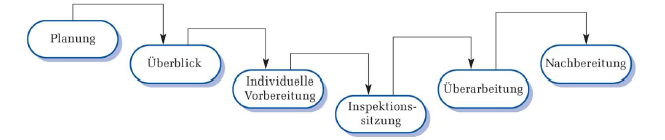
\includegraphics[scale=0.8]{document/graphics/SwInspektion} 
\caption{Sommerville Softwareinspektion}
\end{figure}


\section{Automatisierte statische Analyse}
Bei der Softwareinspektion handelt es sich um eine Form der statistische Analyse. Man verwendet für die Umsetzung oft die Hilfsmittel der Softwareinspektion wie Checklisten und Heuristiken. Hier gibt es ein sehr hohes Automatisierungspotential. 
\\\\
Werkzeuge der statische Analyse helfen bei der Erkennung von Anomalien im Code, wobei nicht jede Anomalie ein Fehler ist. Sie sollten aber alle in einem Review besprochen werden.
\\\\
Es werden Fehlerklassen wie Datenfehler (z.B. uninitialisierte Variablen verwenden,...) Steuerungsfehler (z.B. unerreichbarer Code,..), Ein-Ausgabefehler (z.B. zweimal ausgegebene Variable ohne zwischenzeitliche Zuweisung,..), Schnittstellenfehler (z.B. falsch zugeordnete Parametertypen,..) und Speicherverwaltungsfehler (z.B. nicht zugewiesene Zeiger,..) eingeführt.
\\\\
Bei der statischen Analyse werden verschiedene Phasen abgearbeitet. 
\begin{itemize}
\item Analyse der Steuerung
\item Analyse der Datenverwendung
\item Analyse der Schnittstellen
\item Analyse des Informationsflusses
\end{itemize}

\paragraph{Analyse der Steuerung:} Dies beinhaltet das Erkennen von Schleifen, von unerreichbarem Code  und eine Pfadanalyse für Überdeckungstests.

\paragraph{Analyse der Datenverwendung:} Hier wird überprüft ob nicht initialisierte Variablen gelesen werden, ob nicht gelesene Variablen überschrieben werden, ob Variablen unbenutzt sind oder ob redundante Tests ausgeführt werden.

\paragraph{Analyse der Schnittstellen:} Hier werden die die Anzahl und die Typen der Parameter in Deklarationen und Aufrufen, deklarierte aber nicht aufgerufene Prozeduren und Funktionen sowie nicht verwendete Funktionsergebnisse ermittelt und überprüft.

\paragraph{Analyse des Informationsflusses:} Hier geht es primär um die Erkennung der Abhängigkeiten zwischen Eingabevariablen und Ausgabevariablen.

\subsection{Formale Methoden}
Die Vision ist es formale Methoden als die ultimative statische Verifikationsmethode zu verwenden.
Die Voraussetzung hierfür ist die formale Spezifikation. Der Aufwand hierfür ist allerdings sehr hoch und wird daher praktisch nur für kritische Systeme verwendet. Vielen Kunden fordern dies allerdings inzwischen (z.B. im militärischen Bereich). 
\\\\
Es stehen inzwischen automatische Überprüfungen der Spezifikationen auf Inkonsistenzen und die automatische Generierung von Code aus den Spezifikationen zur Verfügung. 
\\\\
Es gibt allerdings noch einige Probleme. Die Spezifikationen entsprechen meistens nicht den Benutzeranforderungen (Fehler, Lücken,...), da die formalen Spezifikationen oft unverständlich für die Mehrheit der Anwender ist. Die Komplexität sowie der Umfang der Beweise stellt ein weiteres Problem dar. Zudem macht ein oft unzutreffendes Nutzungsmuster die Beweise ungültig.

\subsection{Softwaretest}
Die Softwaretest als Verifikationstechnik ist ein anderes Verfahren zum testen gegen die Spezifikation. Das Ziel ist es Fehler zu erkennen beispielsweise via Whitebox-Tests. Genaueres dazu siehe im Kapitel LV6.

\section{Validierungstechniken}
\subsection{Allgemeine Validierungsmaßnahmen}
Die Allgemeine Validierungsmaßnahmen werden in folgende Phasen unterteilt.
\begin{itemize}
\item Analysephase
\item Entwicklungsphase
\item Validierungsphase
\item Einsatzphase
\end{itemize}

\paragraph{Analysephase:} Die Qualität der Anforderungen werden sichergestellt. Dabei werden Anforderung--Interviews mit einer Vielzahl unterschiedlicher Beteiligter bzw. Betroffener durchgeführt. Anschließend werden Reviews der Anforderungen durch Beteiligte/Betroffene, Experten des Anwendungsgebiets und Experten für Systemeigenschaften durchgeführt.

\paragraph{Entwicklungsphase:} Es werden Design-Reviews mit Beteiligten/Betroffenen durchgeführt. Dabei werden GUI-Prototypen und Interaktionsszenarios vorgestellt.

\paragraph{Validierungsphase:} Es werden Tests mit echte Anwender durch möglichst aller Kategorien durchgeführt. Dabei wird das Feedback z.B. über ein Wiki gesammelt. 

\paragraph{Einsatzphase:} Hier werden Marktbeobachten durchgeführt, Benutzergruppen analysiert und ein Produktwiki gepflegt.

\subsection{Softwaretest}
Auch hier ist es das Ziel die Anwendbarkeit der Software zu überprüfen und das Vertrauen in die Software zu stärken. Genaueres dazu siehe Kapitel LV6.

\subsection{Validierung der Zuverlässigkeit}
Eine weitere Art der Validierung kann über die statische Zuverlässigkeitsmessung erfolgen. Die Probleme bei der statistischen Zuverlässigkeitsmessung sind unter anderem die Unsicherheit über das Betriebsprofil, die Kosten der Testdatenerstellung (eine automatische Generierung ist nicht immer ausreichend) und die statistischen Unsicherheiten.

\section{Validierung der Betriebssicherheit}
Bei der Validierung der Betriebssicherheit kann in folgende Punkte unterteilt werden:
\begin{itemize}
\item Beobachtung
\item Reviews
\item Argumentation der Betriebssicherheit
\item Bedeutung der Prozesse
\end{itemize}

\paragraph{Beobachtung:} Die Zuverlässigkeit lässt sich mittels ROCOF messen. Die Betriebssicherheit jedoch nicht. 

\paragraph{Empfehlung von Reviews:} Dadurch wird unter anderem gewährleistet, dass es eine wartungsfreundliche und verständliche Struktur existiert und die Entwürfe von Algorithmen und Datenstrukturen mit dem spezifizierten Verhalten übereinstimmen.  

\paragraph{Argumentation für Betriebssicherheit:} Hier kann beobachtet werden, dass die formale Verifikation des gesamten Systems eine vollständige Liste aller (auch der externen) Fehler benötigt. Dies ist allerdings unmöglich.  Außerdem ist die Verifikation des gesamten Systems sehr kompliziert, teuer und fehleranfällig. Die Vorgehensweise wäre die formale Definition einer Reihe von Bedrohungen (unsicherer Zustände) in Form von Prädikaten und der Nachweis, dass alle Pfade, die zu einem solchen unsicheren Zustand führen, dem entsprechenden Prädikat widersprechen. 

\paragraph{Bedeutung des Prozesses:} Die Motivation dahinter ist, dass Unfälle zu selten sind um sie mittels statistischen Verfahren unter Kontrolle zu bekommen. Unfälle sind oft nur Verletzungen von "darf nicht"-Anforderungen. Die wichtigsten Aktivitäten in diesem Verfahren sind das Einrichten eines Überwachungssystems, die Zuweisung der Verantwortung an geeignete Personen, die Reviews während des gesamten Prozesses und die Formale Zertifizierung kritischer Komponenten.

\subsection{Validierung der Systemsicherheit}
Motivation für die Validierung der Systemsicherheit  ist das erhalten einer guten Infrastruktur um zu verhindern das von einem beliebigen Rechner auf ein System von uns zugegriffen werden kann. Das Problem dabei ist aber, dass es schwer  Nachzuweisen ist ob ein System keine Fehlfunktionen im Bereich der Sicherheit hat. Um ein gewisses Maß der Sicherheit gewährleisten zu können, gibt es folgende sich ergänzende Überprüfungsansätze:
\begin{itemize}
\item Erfahrungsbasierte Validierung
\item Werkzeugbasierte Validierung
\item Angreiferteams
\item Formale Verifikation
\end{itemize}

Wichtig dabei ist es allerdings zu berücksichtigen, dass keine Kette stärker ist als sein schwächstes Glied.